% Figure: the video-model template. Families C, V01-V08, P03-P04, W01, W05, F03.
% Build: pdflatex fig_video_models.tex
\documentclass[border=2pt]{standalone}
% One look for every architecture figure. Change a colour or font here, once.
\PassOptionsToPackage{table}{xcolor}
\usepackage[T1]{fontenc}
\usepackage{lmodern}
\renewcommand{\familydefault}{\sfdefault}
\usepackage{amsmath}
\usepackage{array}
\usepackage{graphicx}
\usepackage{fontawesome5}
\usepackage{tikz}
\usetikzlibrary{positioning, arrows.meta, fit, backgrounds, calc,
  decorations.pathreplacing}

% colour says where the weights came from, nothing else
\definecolor{preEdge}{RGB}{0,94,150}      % pretrained weights
\definecolor{preFill}{RGB}{214,232,245}
\definecolor{newEdge}{RGB}{176,92,0}      % new weights, trained from scratch
\definecolor{newFill}{RGB}{253,229,196}
\definecolor{opEdge}{RGB}{120,120,120}    % no weights
\definecolor{opFill}{RGB}{236,236,236}
\definecolor{ink}{RGB}{35,35,35}
\definecolor{note}{RGB}{90,90,90}
\definecolor{groupFill}{RGB}{245,245,245}
\definecolor{stripe}{RGB}{243,243,243}
% boxes drawn on photos: Okabe-Ito, readable on grass
\definecolor{strikerBox}{RGB}{0,114,178}
\definecolor{batBox}{RGB}{204,121,167}
\definecolor{cropBox}{RGB}{230,159,0}

% the icon says whether the weights move during training
\newcommand{\frozen}{{\color{ink}\faSnowflake[regular]}}
\newcommand{\trained}{{\color{ink}\faFire}}

% a small filled square for legends; no tikz inside tikz
\newcommand{\swatch}[2]{{\setlength{\fboxsep}{0pt}\setlength{\fboxrule}{0.6pt}%
  \fcolorbox{#1}{#2}{\rule{0pt}{1.4ex}\rule{2.2ex}{0pt}}}}
\newcommand{\archlegend}{\swatch{preEdge}{preFill}~pretrained weights\quad
  \swatch{newEdge}{newFill}~new weights\quad
  \swatch{opEdge}{white}~no weights\qquad
  \frozen~frozen\quad \trained~trained}

% tensor sizes
\newcommand{\by}{\ensuremath{\times}}
\newcommand{\sq}{\textsuperscript{2}}
\newcommand{\dims}[1]{#1}
\newcommand{\arrowto}{\ensuremath{\to}}

\tikzset{
  every node/.style={font=\footnotesize, text=ink},
  flow/.style={-{Stealth[length=2.2mm, width=1.7mm]}, line width=0.75pt,
    draw=ink},
  box/.style={rounded corners=2pt, line width=0.7pt, align=center,
    minimum height=8mm, inner sep=3pt,
    execute at begin node={\hyphenpenalty=10000\exhyphenpenalty=10000}},
  pre/.style={box, draw=preEdge, fill=preFill},
  new/.style={box, draw=newEdge, fill=newFill},
  op/.style={box, draw=opEdge, fill=white},
  group/.style={rounded corners=3pt, draw=opEdge, dashed, line width=0.5pt,
    fill=groupFill, inner sep=4pt},
  grouplabel/.style={font=\scriptsize, text=note, inner sep=1pt},
  % a tensor size, sitting on its arrow so it never crosses a line
  dim/.style={font=\scriptsize, text=ink, fill=white, draw=opEdge!55,
    line width=0.3pt, rounded corners=1.5pt, inner sep=1.1pt},
  size/.style={font=\scriptsize, text=note, inner sep=1.5pt,
    execute at begin node={\hyphenpenalty=10000\exhyphenpenalty=10000}},
  tag/.style={font=\scriptsize\bfseries, inner sep=1pt},
  legend/.style={font=\scriptsize, text=note, inner sep=2pt},
  frame/.style={inner sep=0pt, draw=ink!55, line width=0.3pt},
  letter/.style={font=\footnotesize\bfseries, inner sep=0pt},
  % a box opening up into the table that lists its options
  cone/.style={fill=#1, fill opacity=0.45, draw=none},
  conelink/.style={draw=opEdge!80, line width=0.4pt, densely dashed},
  bone/.style={line width=1.0pt, draw=white, line cap=round},
  guess/.style={line width=0.8pt, draw=white, dash pattern=on 1.6pt off 1.2pt},
  joint/.style={fill=cropBox},
  guessjoint/.style={fill=white},
}

% a clip as a deck of three of its frames; #1 name, #2 where, #3 width
\newcommand{\clipdeck}[3]{%
  \node[frame] (#1-c) at ($(#2)+(0.22,0.22)$)
    {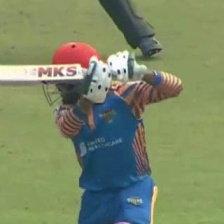
\includegraphics[width=#3]{img/crop15.jpg}};
  \node[frame] (#1-b) at ($(#2)+(0.11,0.11)$)
    {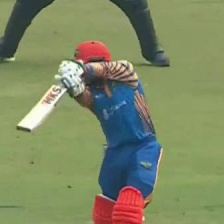
\includegraphics[width=#3]{img/crop08.jpg}};
  \node[frame] (#1-a) at (#2) {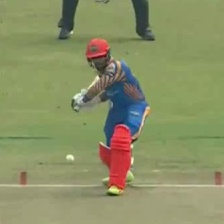
\includegraphics[width=#3]{img/crop01.jpg}};
  \node[fit=(#1-a)(#1-b)(#1-c), inner sep=0pt] (#1) {};
}

% a table card: a header band in the colour of the box it opens up.
% #1 name, #2 top-left corner, #3 band fill, #4 edge, #5 title, #6 a tabular
\newcommand{\card}[6]{%
  \node[anchor=north west, inner sep=0pt, fill=white, font=\scriptsize]
    (#1) at ([yshift=-5mm]#2) {#6};
  \node[fit={(#1.north west)([yshift=5mm]#1.north east)}, inner sep=0pt,
    fill=#3] (#1-head) {};
  \node[anchor=west, inner sep=0pt, font=\footnotesize\bfseries]
    at ([xshift=4pt]#1-head.west) {#5};
  \draw[#4, line width=0.7pt] (#1-head.north west) rectangle (#1.south east);
  \draw[#4, line width=0.5pt] (#1-head.south west) -- (#1-head.south east);
}
% rows inside a card
\newcommand{\cardrule}{\arrayrulecolor{opEdge!60}\hline}
\newcommand{\grouprow}[2]{\rowcolor{white}%
  \multicolumn{#1}{l}{\rule{0pt}{2.6ex}\textbf{\color{note}#2}}\\}
\newcolumntype{P}[1]{>{\raggedright\arraybackslash}p{#1}}
\newcommand{\cardtable}[2]{{\setlength{\tabcolsep}{4pt}%
  \hyphenpenalty=10000\exhyphenpenalty=10000%
  \renewcommand{\arraystretch}{1.12}\rowcolors{2}{white}{stripe}%
  \begin{tabular}{#1}#2\end{tabular}}}
% the shaded zoom from a box (#1) down to its card (#2), colour #3
\newcommand{\zoomto}[3]{%
  \begin{scope}[on background layer]
    \fill[cone=#3] (#1.south west) -- (#1.south east) --
      (#2-head.north east) -- (#2-head.north west) -- cycle;
  \end{scope}
  \draw[conelink] (#1.south west) -- (#2-head.north west);
  \draw[conelink] (#1.south east) -- (#2-head.north east);
}


\begin{document}
\begin{tikzpicture}

% ---- (a) colour: the clip as a whole ----
\node[letter, anchor=south west] (la) at (0,1.12) {(a)\enspace The whole clip at once};
\clipdeck{clip}{0.8,0}{1.35cm}

\node[op, text width=2.1cm, right=1.05cm of clip] (fit)
  {\textbf{Match the weights}\\[1pt]
   {\scriptsize resample the frames, resize, recolour}};
\node[pre, text width=2.35cm, right=1.5cm of fit] (bb)
  {\textbf{Video backbone}\\[1pt]
   {\scriptsize Kinetics-400; space and time together}};
\node[new, text width=1.85cm, right=1.3cm of bb] (cls)
  {\textbf{Classifier}\\[1pt]
   {\scriptsize new linear layer, or an MLP}};
\node[right=0.45cm of cls, align=center, inner sep=1pt] (out)
  {\textbf{Cover}\\\textbf{Drive}\\[-1pt]{\scriptsize\color{note}top score}};

\draw[flow] (clip.east |- fit.west) -- node[dim] {15\by224\sq} (fit.west);
\draw[flow] (fit) -- node[dim] {\textit{T}\by\textit{S}\sq} (bb);
\draw[flow] (bb) -- node[dim] {1\by\textit{D}} (cls);
\draw[flow] (cls) -- (out);

\card{cb}{$(fit.south west)+(-0.45,-1.15)$}{preFill}{preEdge}
  {Video backbones: their input, and how each was used}{%
\cardtable{l c c c c c}{%
\rowcolor{white} & frames & size & \trained\ fine-tuned, & \frozen\ frozen, & \frozen\ frozen,\\
\rowcolor{white} & \textit{T} & \textit{S}, px & new linear & MLP & one linear\\ \cardrule
\grouprow{6}{3D CNNs}
R3D-18 & 15 & 112 & C02 & V01 & P03\\
MC3-18 & 15 & 112 & & V02 & \\
R(2+1)D-18 & 15 & 112 & C01 & V03 & \\
S3D & 15 & 224 & & V04 & \\
I3D-R50 & 8 & 224 & C03 & & \\
SlowFast-R50 & 32\,+\,8\textsuperscript{1} & 224 & C04 & & \\
X3D-M & 16 & 224 & C05 & & \\
\grouprow{6}{Video transformers}
MViTv2-S & 16 & 224 & C06 & V06 & \\
Swin3D-T & 15 & 224 & C07 & V05 & \\
VideoMAE-B & 16 & 224 & C08 & V07 & P04\\
TimeSformer-B & 8 & 224 & & V08 &
}}
\node[size, anchor=north west, text width=8.6cm, align=left] (fn)
  at ([yshift=-0.5mm]cb.south west)
  {Our 15 frames become 16 by repeating the middle one, and 8 by keeping
   every other one. \textsuperscript{1}\,SlowFast reads the clip twice:
   32 frames on its fast path, 8 on its slow one.};
\zoomto{bb}{cb}{preFill}

% ---- (b) motion instead of colour ----
\node[letter, anchor=north west] (lb) at ($(0,0 |- fn.south)+(0,-0.55)$)
  {(b)\enspace Motion instead of colour};
\clipdeck{clip2}{$(lb.south west)+(0.8,-1.75)$}{1.35cm}
\node[pre, text width=2.75cm, align=left, font=\scriptsize, anchor=south] (flow)
  at ([yshift=0.8mm]fit |- clip2.center)
  {\textbf{\footnotesize Optical flow}\hfill\frozen\\RAFT-small; 2 channels};
\node[op, text width=2.75cm, align=left, font=\scriptsize, anchor=north] (diff)
  at ([yshift=-0.8mm]fit |- clip2.center)
  {\textbf{\footnotesize Frame differences}\\each frame minus the one before; 3 channels};
\begin{scope}[on background layer]
  \node[group, fit=(flow)(diff), inner sep=4pt] (motion) {};
\end{scope}
\node[grouplabel, anchor=south] at (motion.north) {one of};
\node[pre, text width=2.35cm, at=(bb |- motion)] (r3d)
  {\textbf{R3D-18}\\[1pt]
   {\scriptsize Kinetics-400; first conv.\ rebuilt for 2 or 3 channels}\\[1pt]
   {\scriptsize\trained}};
\node[new, text width=1.85cm, at=(cls |- motion)] (cls2)
  {\textbf{New linear}\\[1pt]{\scriptsize 512\,\arrowto\,15}};
\node[align=center, inner sep=1pt, at=(out |- motion)] (out2)
  {\textbf{Cover}\\\textbf{Drive}};
\draw[flow] (clip2.east |- motion.west) -- (motion.west);
\draw[flow] (motion) -- node[dim] {14\by112\sq} (r3d);
\draw[flow] (r3d) -- node[dim] {1\by512} (cls2);
\draw[flow] (cls2) -- (out2);

\node[size, anchor=north west, align=left, text width=4.3cm] (wids)
  at ([yshift=-2.5mm]motion.south west)
  {\textbf{\color{ink}W01} optical flow,\enspace \textbf{\color{ink}W05} frame
   differences. Flow is computed at 224~px, then shrunk to 112.};
\node[op, text width=4.5cm, align=left, font=\scriptsize, anchor=north east]
  (f03) at ([yshift=-2.5mm]out2.east |- r3d.south)
  {\textbf{\footnotesize F03, two streams:} the probabilities of C02 (colour)
   and W01 (flow) averaged; no new weights};

% ---- legend ----
\node[legend, anchor=north] at ($(current bounding box.south)+(0,-1.5mm)$)
  {\archlegend\qquad \textit{D}: clip-vector length};
\end{tikzpicture}
\end{document}
